\setcounter{section}{47}
\section{Алгоритм Дейкстры. Условия применимости, доказательство корректности. Реализации за $O(n^2), O(m \log n)$, 
$O(m + n \log n)$.}

Алгоритм Дейкстры ищет кратчайшие пути в графе от заданной вершины до всех, если веса всех ребер неотрицательны.

В алгоритме поддерживается множество вершин $U$ (использованных вершин), для которых уже вычислены длины кратчайших путей до них из $s$. На каждой итерации основного цикла выбирается вершина $u \notin U$, которой на текущий момент соответствует минимальная оценка кратчайшего пути. Вершина $u$ добавляется в множество $U$ и производится релаксация по всем исходящим из неё рёбрам. Релаксация~--- процесс, в котором мы обновляем расстояния до вершин, смежных с $u$ и не принадлежащих $U$. 

\lstinputlisting[language=C++,
emph={int,char,double,float,unsigned},
emphstyle={\color{blue}}
]{code/48_deikstra.cpp}

По сути, $0-k-bfs$ работает точно так же.

В такой наивной реализации асимптотика $O(n^2)$, если искать минимальную неиспользованную вершину за линию.\\

Можно добиться $O(m \log n)$, используя двоичную кучу. А что нам, в сущности, нужно? Искать минимум на неиспользованных вершинах и уменьшать значения (extract min и decrease key). Куча такое как раз умеет.

С фиб. кучей асимптотика будет даже лучше. Будет $O(m + n \log n)$, поскольку в фиб куче decrease key выполняется амортизированно за 1.

\begin{theorem}[Корректность]
Докажем, что если $v$ раскрываемая вершина, то $dist[v] = dist(s, v)$. Отсюда будет следовать корректность.
\end{theorem}

\begin{proof}
Пусть это не так. Найдем первую вершину $v$, для которой это не выполняется. Это может быть только в случае, если $dist[v] > dist(s, v)$. Тогда исходя из алгоритма $dist[u] \geq dist[v]$ для всех неиспользованных $u$.\\

Как может выглядеть кратчайший путь от $s$ до $v$? Он выглядит так. Мы сначала ходим по использованным вершинам, а потом прыгаем в некоторую вершину $u$ из неиспользованных. А дальше идем в $v$. Пусть $u = v$. Тогда в этом случае такой путь должен был быть учтен в $dist[v]$, когда мы раскрывали вершину, из которой и совершается прыжок. Поэтому получаем, что кратчайший путь до $v$ так выглядеть не может.

Значит, $u \neq v$. Тогда (исходя из предыдущих рассуждений) $dist(s, u) = dist[u] \geq dist[v] > dist(s, v) > dist(s, u)$. (Ведь $dist(s, v) = dist(s, u) + dist(u, v)$). Получаем противоречие. Ура.
\end{proof}

\setcounter{section}{48}
\section{Двусторонний алгоритм Дейкстры. Завершение алгоритма: почему достаточно реализовать алгоритм, почему нельзя обойтись меньшим числом действий (пример).}

Нужно найти кратчайшее расстояние между $s$ и $t$.
Идея такая же, как в двустороннем bfs. Одновременно идем алгоритмом из вершины $s$ и из вершины $t$ (только в случае вершины $t$ снова рассматриваем обратные ребра).
Как только встретится общаа вершина, радуемся.\\

Собственно, для этих целей нам нужно завести две кучи -- для $s$ и для $t$. Каждый раз будем выбирать минимум из двух куч. Если минимум в куче вершины $s$, то делаем шаг алгоритма Дейкстры для нее, иначе -- для $t$. Останавливаемся, когда какая-то вершина будет удалена из обеих куч.

Тонкость этого алгоритма заключается в том, что кратчайший путь $s \rightarrow t$ не обязательно пройдёт через вершину $mid$ (которая будет удалена из обееих куч). Поэтому после остановки двунаправленного поиска, нам необходимо перебрать некоторое количество ребер.
И ответ в этом случае будет $min$ $dist_s[u] + cost(u, v) + dist_t[v]$ по ребрам $(u, v) \in E$, где имеет смысл перебирать только ребра между теми вершинами, которые были посещены во время нашего обхода ($u$ посещалась алгоритмом для $s$, а $v$ -- для $t$).

На практике, такой двунаправленный поиск быстрее обычного алгоритма Дейкстры примерно в два раза.

\textbf{Пример.} Почему через $mid$ не всегда проходит нужный путь.

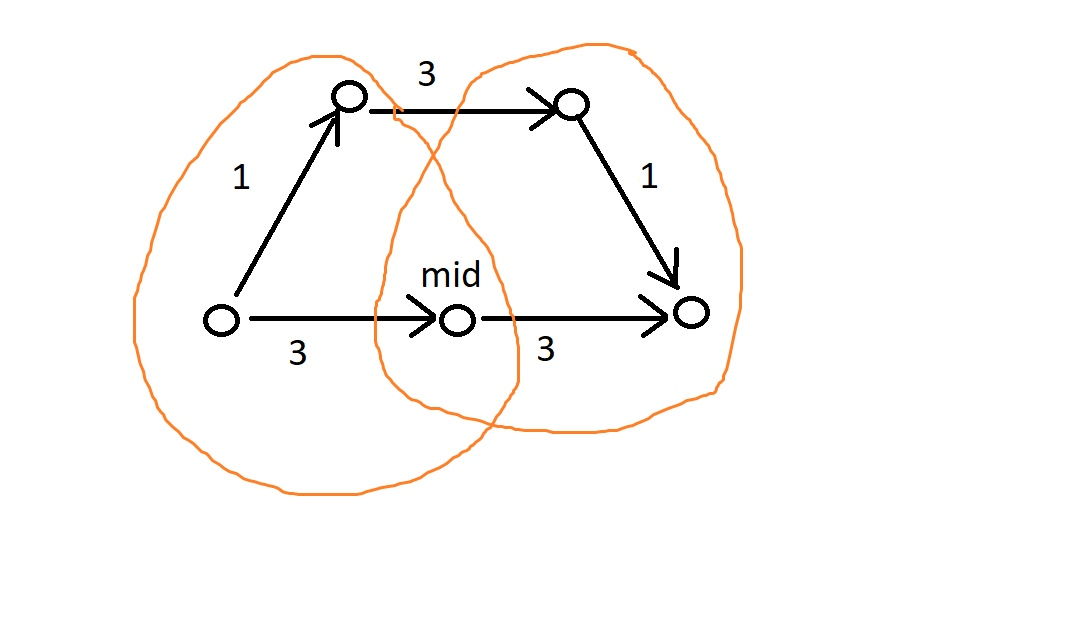
\includegraphics[width=0.5\textwidth]{images/49.jpg}\\

\textbf{Почему достаточно перебрать такие ребра.}\\

Пусть $s \to u \to v \to t$ -- путь, который нашел наш алгоритм. Где $u$ -- из "облачка" вершины $s$, а $v$ -- из "облачка" $t$. (Облачко -- посещенные вершины).

$mid$ -- пересечение облачков.

Пусть мы не учли какой-то путь. Тогда он выглядится так. Мы пошли по вершинам из облачка $s$, дальше походили по вершинам, не принадлежащим никакому облачку, потом походили как-то еще, а потом прошлись по вершинам из облачка $t$. Пусть $x$ и $y$ -- первая и последняя вершны не из облачков.\\

Тогда $dist(s, x) \geq dist(s, mid)$, $dist(y, t) \geq dist(mid, t)$. Значит, на самом деле, такой путь нам неинтересен.